\scanpage{80}
\margin{\figure{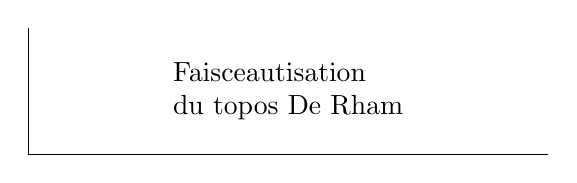
\begin{tikzpicture}
\node[align=left] at (3.3,.6) {Faisceautisation\\du topos De Rham};
\draw (0,1.4)--(0,-.2)--(6.6,-.2);
\end{tikzpicture}}}
1. Soit $X$ un topos, et
\[
\mathbb Z\xrightarrow{u}\Phi
\]
une immersion de $\mathbb Z$ dans un faisceau $\Phi$, tel que

a) $\operatorname{Coker}\Phi$ est $\mathbb Z$-plat

b) Pour tout $i>0$, $\Lambda_{\mathbb Z}^i\Phi$ et $\Gamma_{\mathbb Z}^i\Phi$ sont flasques, et le restent par tensorisation avec tout faisceau abélien.

En particulier, on en conclut \deleted{par récurrence et dévissage} que \deleted{\unsure{si}}
b') Si $i,j\geq0$ et $i+j>0$, alors $\deleted{\unsure{\Lambda}}\Gamma_{\mathbb Z}^i\Phi\otimes\Lambda_{\mathbb Z}^j\Phi$ est flasque.

De b') on conclut \deleted{que}\inserted{(par récurrence et dévissage)}, posant
\[
\operatorname{Coker}i=\Psi
\]
\inserted{que}
$\alpha)$ les $\Gamma_{\mathbb Z}^i\Phi\otimes\Lambda_{\mathbb Z}^j\Psi$ sont flasques pour $i>0$. !

De $\alpha$ on conclut \deleted{\unsure{que}}:

$\beta)$ Posant $K_u^{\bullet\bullet}=\Gamma_{\mathbb Z}^*\Phi\otimes\Lambda_{\mathbb Z}^*\Psi$,
avec l'op. diff. \deleted{\unsure{d}} $d$ compatible aux puissances divisées qui,
sur $\deleted{\unsure{\Gamma^0\otimes\Lambda^1}}\Psi$ est nul et sur $\unsure{\widehat\Phi|\Phi}$ est l'hom canonique $\Phi\longrightarrow\Psi$, et définissant
\[
\mathbb Z\{T\}\longrightarrow H^{*0}(K_u^{**})
\]
par $T\longmapsto1\in\mathbb Z=\operatorname{Ker}(\Phi\xrightarrow{d}\Psi)$,
et prolongeant par la condition d'être compatible aux p.div,
on trouve que $K_u^{\bullet\bullet}$ est une \uline{résolution} de $\mathbb Z\{T\}$.

Utilisant encore a), \inserted{et b)}, on trouve

$\gamma)$ Pour tout faisceau d'anneaux comm. $k$ sur $X$,
$K_{u,k}^{\bullet\bullet}\simeq K_u^{\bullet\bullet}\otimes k
\simeq\Gamma_k^*\Phi_k\otimes\Lambda_k^*\Psi_k$ est une résolution de
$k\{T\}\simeq H^{\bullet0}(K_{u,k}^{\bullet\bullet})$, et les
$\Gamma_k^i\Phi_k\otimes\Lambda_k^j\Psi_k$ sont flasques pour $i>0$.
\margin{79}
